\chapter{Post-Processing Techniques for Instance Segmentation Masks}\label{ch:postProcessing}

At this stage, the system is capable of detecting cetaceans at an individual pixel level. Before these detections can be passed to the identification module, some post-processing of the output must be performed to allow for both a reduction in the computational expense of operating on the detector's output as well as ensuring that no potentially important information which will assist in an identification is lost. 


\section{Background Subtraction \& Cropping}\label{ch:postProcessing,sec:bgExtraction}

One of the main components of the post-processing pipeline is the background subtraction module. This is an extremely important step in ensuring an accurate individual classification based on the detected fin. By removing the surrounding background from around the fin, this reduces the amount of noise the identifier will be required to deal with. Thanks to the segmentation masks produced by the Mask-RCNN detector \cite{he_mask_2017} in Chapter \ref{ch:cetDet}, the pixels which are likely background have been identified.

As both the input image and its resultant mask can be represented as matrices, these can be manipulated utilising a \textit{bitwise and} operation such that if pixel$_{i, j}$ in the input image is denoted as background in the mask, the values of pixel$_{i, j}$ can be set to [255, 255, 255] (white). This has the effect of whiting out any pixels not detected as part of the fin in the image, removing noise. 

Once the background subtraction has been achieved the input image can then be cropped to reduce file size. By using the top, bottom, left, and right-most non-white pixels in the image as bounding box coordinates for the fin, the input image can be vastly reduced, often to only a few hundred pixels in both height and width. This greatly reduces the computational expense of further operations downstream by reducing the size of subsequent input images passed to other components. 

Figure \ref{fig:fin-extraction-clean} shows the effect of performing background subtraction on an input image, with the detected \texttt{dolphin} pixels from the Mask-RCNN highlighted in red. As can be seen, the background subtraction and cropping has resulted in a clean image of the animal's dorsal fin. Identifying information is present, with minimal levels of noise. 

\begin{figure}[h]
	\begin{center}
		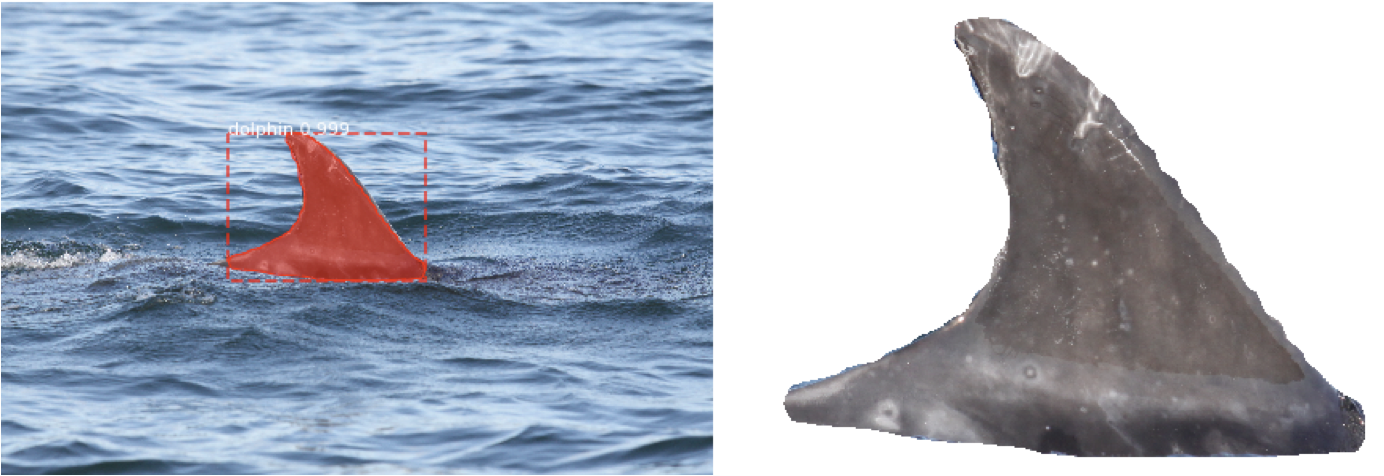
\includegraphics[scale=0.5]{Chapter4/figs/fin-extraction-clean.png}
	\end{center}
	\caption{The effect of background subtraction and cropping on an input image, left. The detected \texttt{dolphin} pixels by the Mask-RCNN have been highlighted in red with confidence score shown. The resultant output, right, has been enlarged for visibility.}
	\label{fig:fin-extraction-clean}
\end{figure}

Whilst the background subtraction module aims to reduce as much noise as possible entering the identification module, which can be achieved thanks to the high accuracy of the detector, it will not be possible to remove all noise. It may be the case, such as in Figure \ref{fig:fin-extraction-unclean}, whereby some background has been mislabelled as \texttt{dolphin}. As a result, the background subtraction module is unable to remove the mislabelled background pixels which may effect the accuracy of the identification downstream unless the system is robust enough to deal with this.

\begin{figure}[h]
	\begin{center}
		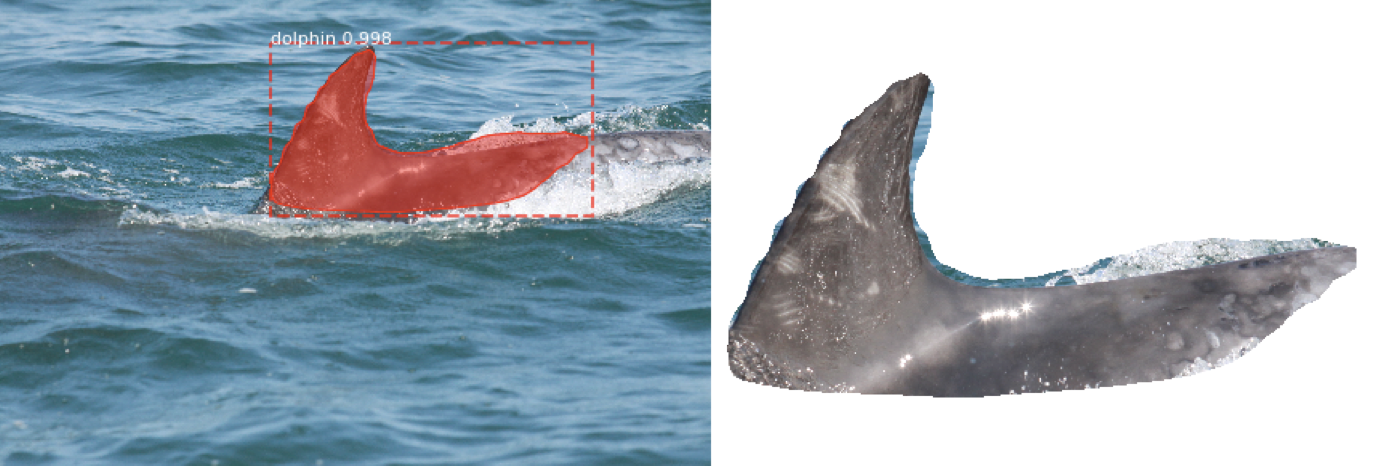
\includegraphics[scale=0.5]{Chapter4/figs/fin-extraction-unclean.png}
	\end{center}
	\caption{The result of background subtraction and cropping where the detector has mislabelled some background pixels as \texttt{dolphin}, right. Detected pixels have been highlighted red on the input image, left, with confidence score shown.}
	\label{fig:fin-extraction-unclean}
\end{figure}

As cetaceans often travel in pods containing multiple individuals, any post-processing methodology must be capable of handling this. To account for this, if the background subtraction module is passed multiple masks for an image it operates on each mask independently. This results in potentially multiple output images per input, one for each detection. An example of this behaviour can be seen in Figure \ref{fig:fin-extraction-pod-with-flag}.

\begin{figure}[h]
	\begin{center}
		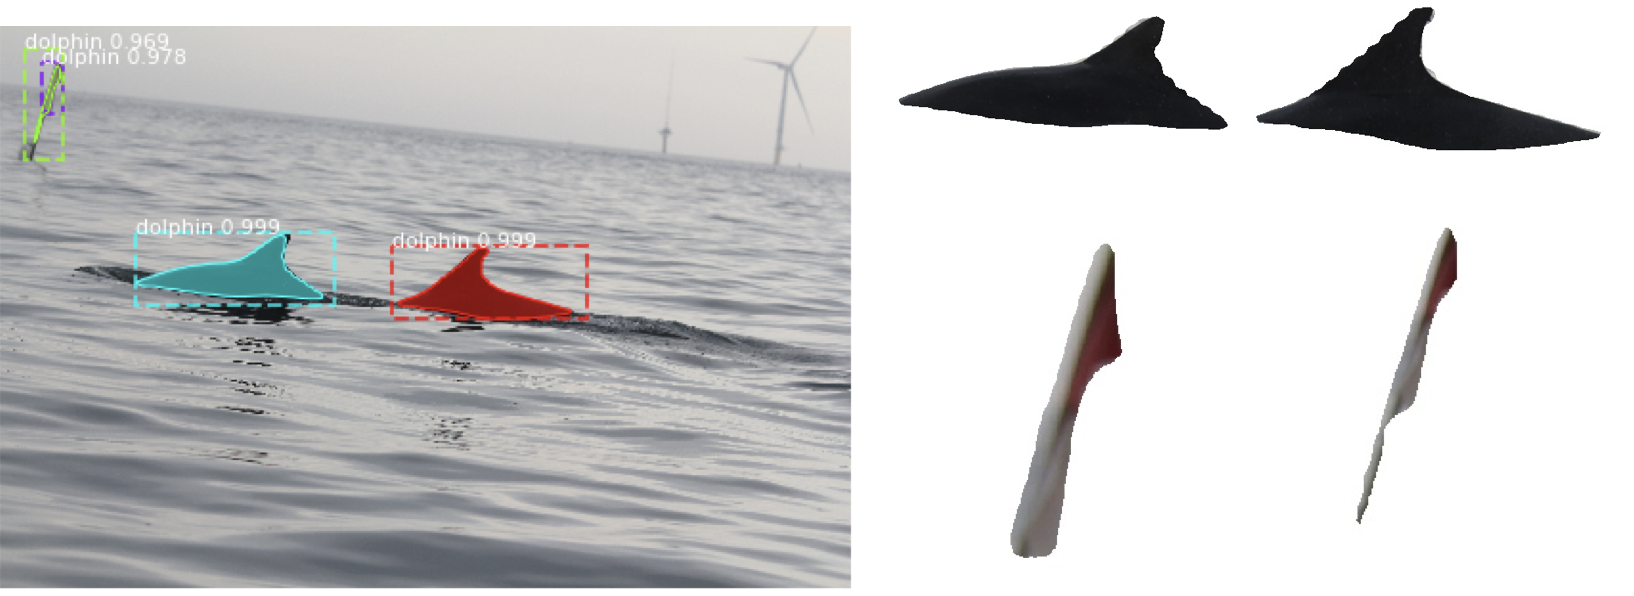
\includegraphics[scale=0.5]{Chapter4/figs/fin-extraction-pod-with-flag.png}
	\end{center}
	\caption{The result of background subtraction and cropping where the detector is passed multiple masks for an input image, right. Detections and confidence scores are overlaid onto the input image, left.}
	\label{fig:fin-extraction-pod-with-flag}
\end{figure}

As the Mask-RCNN has detected four \texttt{dolphin} objects in the image, the background subtraction and cropping module has produced four output images. However it can be seen that two of the detections have been misclassified - they are actually of a flag denoting the location of a lobster pot and thus should be background. Further post-processing of the detection outputs is required to ensure the minimal amount of erroneous detections are passed downstream without stopping correct classifications. 

\section{Morphological Transformations}\label{ch:postProcessing,sec:morphologicalTransformations}

Before the \textit{bitwise and} operation described in Section \ref{ch:postProcessing,sec:bgExtraction}, a further post-processing technique known as morphological transformations can be performed. These are a set of operations which allow for the automated manipulation of the internal structure of an in a binary image. 

The two fundamental morphological transformations are called erosion, which erodes away the boundaries of the masked object, and dilation, which increases the size of the object by pushing the boundary out into the background space. These two operations can be utilised in various combinations to perform other useful transformations.

In some situations, the detector may produce a mask which contains an unwanted internal hole. As the pixels inside this hole would be considered background they are removed by the background subtraction module, resulting in potentially lost identifying individual information. To prevent this from occurring, each detected mask is \textit{closed} - dilated then eroded. This has the effect of removing any holes present inside the mask. If no holes exist, the operation is still performed however the mask remains unchanged. By performing closing, the system ensures that no potentially identifiable information is lost at this stage. 

An example closing operation can be seen in Figure \ref{fig:before-and-after-morphing}. The top row shows the mask for an input image, with \texttt{dolphin} highlighted in white, as well as the resultant output image after background subtraction. Note the hole in the mask and resultant output image. The bottom row shows the same mask and output image after closing has been applied. Note the hole has now been filled in the mask, and the information which would have been lost has now been preserved in the output.

\begin{figure}[h]
	\begin{center}
		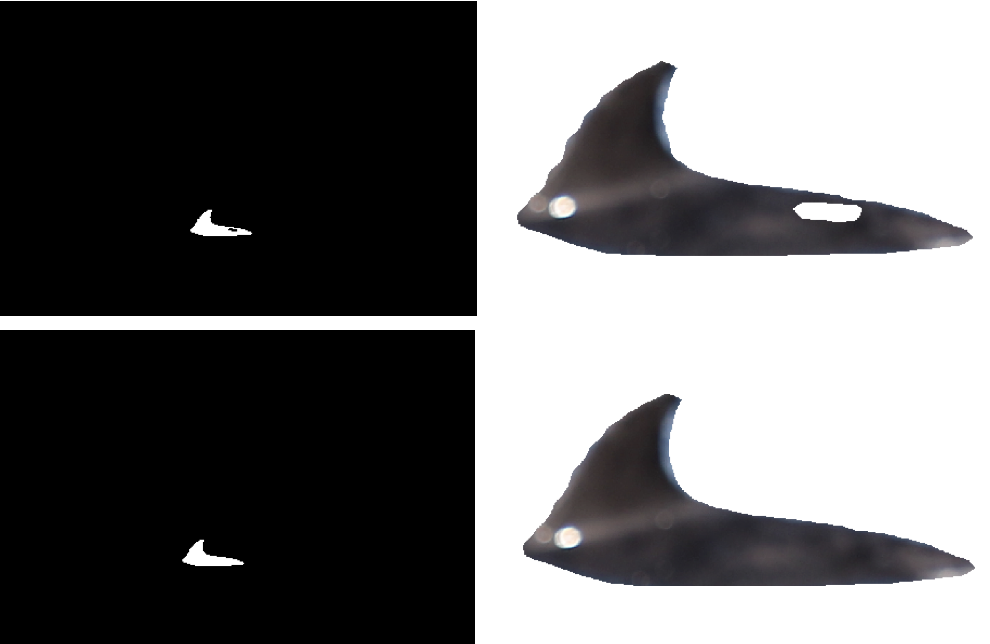
\includegraphics[scale=0.5]{Chapter4/figs/before-and-after-morphing-masks.png}
	\end{center}
	\caption{Top: Detected mask output with \texttt{dolphin} highlighted in white and the resultant output image without closing. Bottom: The same mask and output image but closing has been applied.}
	\label{fig:before-and-after-morphing}
\end{figure}


% Rejig this chapter to follow format in Log 16/3


%%%%%%%%%%%%%%%%%%%
\nomenclature[z-CNN]{CNN}{Convolutional Neural Networks}

